\section{Introduction}

The main goal of the present work is to develop an efficient open-source library in C++ for the numerical modelling of natural gas transport through a long-distance network. Additional requirements   as steady and unsteady state simulations, mixture of gases to take into account hydrogen blending for instance. Previous open-source tools can be find in the literature. Let us mention open-sources available in the literature as GasNetSim, pandapipes and MORGEN. The first was presented recently in \url{https://ieeexplore.ieee.org/document/9769148}, where authors argued GasNetSim is the first open-source tool that allows complex mixture composition of gases. This salient advantage can be only exploited for steady regime till now. The second library has less model flexibility and, as in in the former, is written Python.on. The latter stands for Model Reduction for Gas and Energy Networks, which is an academic tool developed in Matlab based on the isothermal Euler equations. \cred{[CONTRIBUTION REQUIRED FROM DENERG]}  

\subsection{Architecture of shimmer++} 
The open-source tool is based on the architecture scheme shown in Fig. \ref{intro:architecture} with a disk-representation, a in-memory representation, and a numerical methods stage. Its parts and the boundaries in between will be presented in detail in the following sections.
\begin{figure}[H]
    \centering
    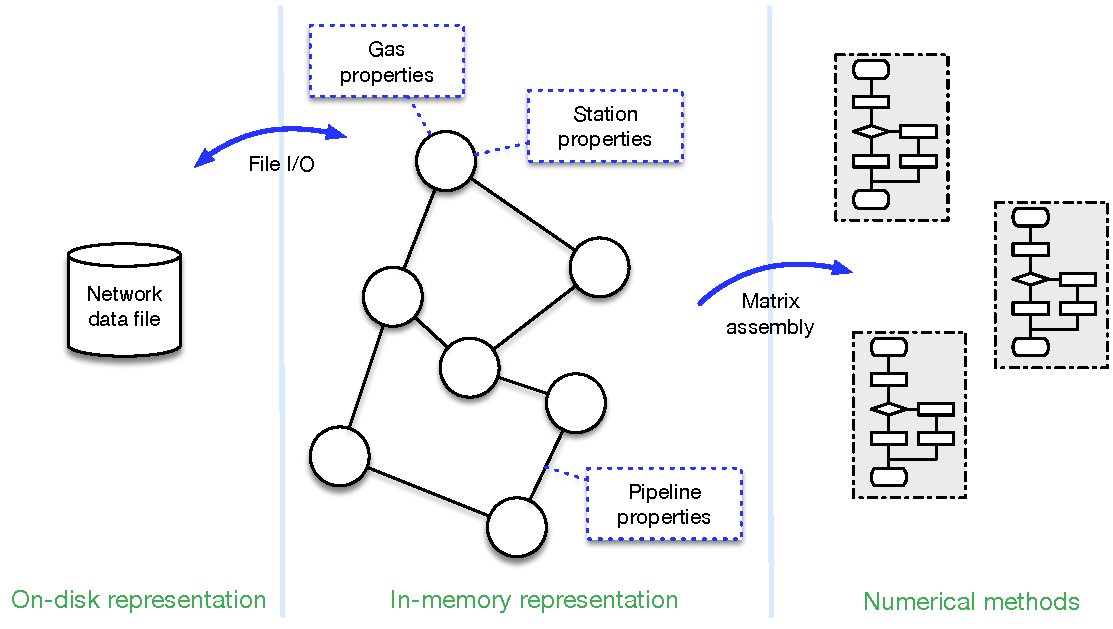
\includegraphics[scale = 0.7]{img_intro/system_arch.pdf}  
    \caption{System architecture scheme.}
    \label{intro:architecture}
\end{figure}

